\section{Datasets in Federated Learning Research}
%%%%%%%%%%%%%%%%%%%%%%%%%%%%%%%%%%%%%%%%%%%%%%%%%%%%%%%%%%%%%%%%%%%%%%%%%%%%%%%
Datasets comprise a fundamental factor in machine learning, including fields such as Federated Learning. Essentially, they offer
training samples along with their corresponding labels, providing the algorithm with the necessary input to be able to extract
underlying model patterns, relationships, and representations essential for accurate and efficient generalization. A good dataset
for machine learning needs to satisfy the following requirements:

\begin{figure}[!ht]
    \centering
    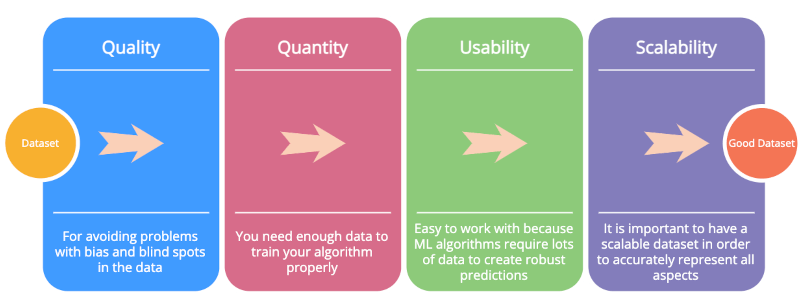
\includegraphics[width=\textwidth]{figures/datasets/good_dataset.png}
    \caption{Features of a good dataset for machine learning}
    \label{fig:good_dataset}
\end{figure}

Quality samples in datasets are accurate, reliable, and contain a balanced distribution among the data classes, ensuring that the model
learns from trustworthy and informative examples. Quantity is necessary with ML algorithms requiring a vast number of samples to achieve
generalization, offering diverse coverage of the underlying data distributions to avert overfitting and achieve convergence. Usability
refers to the dataset being properly formatted and accompanied by clear metadata facilitating seamless utilization by researchers and
practitioners. Finally, scalability is required to be able to accommodate varying volumes of data without compromising performance or efficiency.
%%%%%%%%%%%%%%%%%%%%%%%%%%%%%%%%%%%%%%%%%%%%%%%%%%%%%%%%%%%%%%%%%%%%%%%%%%%%%%%
\subsection{Benchmark Datasets}

The process of creating a proper dataset for machine learning tasks, especially in the context of federated learning, is non-trivial.
It involves meticulous curation, preprocessing, and validation to ensure that the dataset accurately represents the underlying data distribution
and facilitates meaningful model training. Given the complexity and challenges associated with dataset creation, several benchmark datasets
are utilized in the FL community to evaluate the performance of federated learning algorithms. Some examples relevant to our research's
implementation are presented:

\begin{itemize}
    \item \textbf{MNIST}: MNIST is a dataset of handwritten digits widely used for image classification tasks.
          It consists of $28 \times 28$ grayscale images of digits from 0 to 9, with corresponding labels.
    \item \textbf{Fashion-MNIST}: Fashion-MNIST is a dataset of clothing articles used for image classification tasks, similar to
          MNIST but with more diverse classes. It consists of $28 \times 28$ grayscale images of fashion items such as shirts, shoes, and trousers.
    \item \textbf{CIFAR-10}: CIFAR-10 is a dataset of small images across ten classes, often used for image recognition tasks.
          It contains 60,000 $32 \times 32$ color images, with 6,000 images per class.
    \item \textbf{CIFAR-100}: CIFAR-100 is an extension of CIFAR-10, containing 100 classes of objects. It provides a more challenging
          classification task compared to CIFAR-10, with finer-grained categories.
\end{itemize}

These benchmark datasets serve as standardized tasks for evaluating federated learning algorithms, allowing researchers to assess model performance
across different domains. By utilizing well-established datasets like MNIST, CIFAR-10, Fashion-MNIST, and CIFAR-100, researchers can compare the
effectiveness of their FL implementations, measure their generalization capabilities, and identify areas for improvement in federated learning
methodologies. In that spiit, these datasets were preferred in our study.

\begin{figure}[!ht]
    \centering
    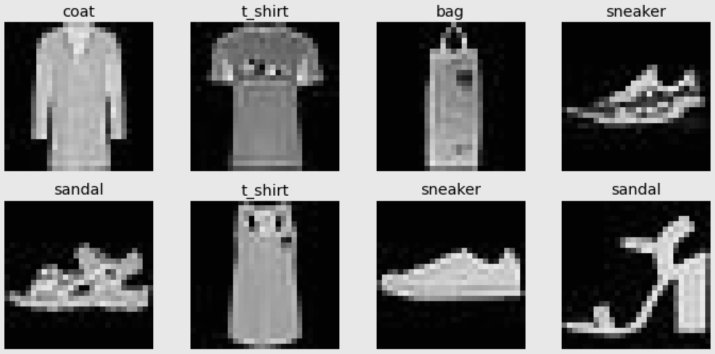
\includegraphics[width=.8\textwidth]{figures/datasets/fashion_mnist.png}
    \caption{Illustration of Fashion-MNIST samples}
    \label{fig:mnist_dataset}
\end{figure}


%%%%%%%%%%%%%%%%%%%%%%%%%%%%%%%%%%%%%%%%%%%%%%%%%%%%%%%%%%%%%%%%%%%%%%%%%%%%%%%
\subsection{Real-world Datasets}
While benchmark datasets offer controlled environments for evaluating federated learning algorithms, real-world datasets
present unique challenges and opportunities, essential for real-life Federated System implementations. Benchmark datasets
provide some intuition about system performance but do not encompass fundamental issues characteristic of realistic scenarios,
such as heterogeneous distribution, data privacy regulations, and continuous data generation.

As Federated Learning expands into real-life applications in \emph{healthcare}, \emph{mobile apps}, and \emph{finance}, the
need for appropriate datasets for these applications increases. Examples include:

\begin{itemize}
    \item \textbf{Healthcare Data}: Patient records, medical images, and sensor data collected from various healthcare institutions.
    \item \textbf{IoT Data}: Sensor readings, device logs, and telemetry data generated by Internet-of-Things (IoT) devices.
    \item \textbf{Financial Data}: Transaction records, credit scores, and market data from banking and financial institutions.
\end{itemize}

%%%%%%%%%%%%%%%%%%%%%%%%%%%%%%%%%%%%%%%%%%%%%%%%%%%%%%%%%%%%%%%%%%%%%%%%%%%%%%%
\subsection{IID VS.\ non-IID Data Distributions}
Two crucial methods of data distribution can be identified in decentralized learning settings.
\paragraph{Independent and Identically Distributed (IID)} In an IID data distribution, each client's data is drawn from the same underlying
distribution, and the data samples are independent of each other. That is to say, each sample is drawn independently from the same
probability distribution and exhibits identical statistical properties with the rest, representing the overall population distribution.

\paragraph{Non-IID} Non-IID data distributions occur when each client's data sample follows a different distribution, either due to variations in data
sources, data collection methods, or client-specific characteristics.

In many traditional \emph{distributed machine learning systems} research, IID data distributions
are frequently assumed, where the central server decentralizes data in such a manner that each client possesses a representative subset
of the overall dataset. However, this assumption often overlooks the inherent complexities of real-world data distributions, especially
in federated systems. In federated learning, where data remains decentralized across multiple clients, achieving true IID data distributions
is often impractical or unrealistic.

\begin{figure}[!ht]
    \centering
    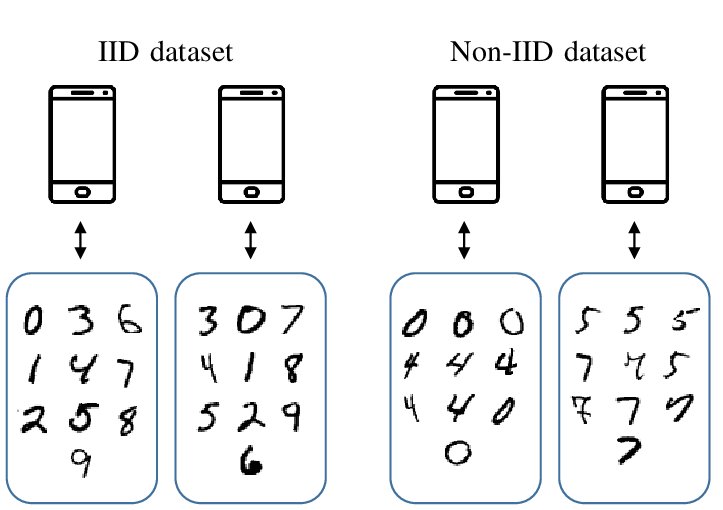
\includegraphics[width=.6\textwidth]{figures/datasets/iid_vs_noniid.png}
    \caption{Example of IID and non-IID distributions of MNIST:\ In the IID dataset,
        each device contains a similar and random sample of digits $(0-9)$, ensuring that
        the data distribution on each device is similar to the overall distribution. In
        the Non-IID dataset, each device contains digits that are not uniformly distributed;
        instead, each device has a concentration of certain digits. For example, one device
        has mostly 0s, another mostly 7s, and so on}
    \label{fig:label}
\end{figure}

In federated learning, data distributions across clients can significantly impact the training process and model performance, thus,
both cases should be studied. IID distributions provide a simplified benchmark for evaluating federated learning algorithms, while
non-IID reflect the inherent heterogeneity in practical deployments. The conjunction of the two, in conclusion, ensures that
federated learning algorithms are not only theoretically sound but also practical and effective in real-world settings.
%%%%%%%%%%%%%%%%%%%%%%%%%%%%%%%%%%%%%%%%%%%%%%%%%%%%%%%%%%%%%%%%%%%%%%%%%%%%%%%